\documentclass[12pt,a4paper,twoside]{article}
\usepackage{labor}
\begin{document}

%fill for cover and header creation
\newcommand\laboratorynumber{2}
\title{Fallrohr}
\newcommand\supervisor{Ditlbacher, Harald}
\newcommand\groupnumber{42}

\newcommand\participantonelastname{Eisner}
\newcommand\participantonefirstname{Nico}
\newcommand\participantoneid{12214121}
\newcommand\participanttwolastname{Waldl}
\newcommand\participanttwofirstname{Philip}
\newcommand\participanttwoid{12214120}
\author{\participantonelastname \ \& \participanttwolastname}

\newcommand\degreeid{UB 033 678}
\newcommand\semester{23WS}
\date{11.11.2023}

%select correct course title
%\newcommand\coursetitle{Einführung in die \\ physikalischen Messmethoden}
%\newcommand\coursetitle{Laborübungen 1: \\ Mechanik und Wärme}
\newcommand\coursetitle{Laborübungen 2: \\ Elektrizität, Magnetismus, Optik}
%\newcommand\coursetitle{Fortgeschrittenen Praktikum 1: \\ Technische Physik}
%\newcommand\coursetitle{Fortgeschrittenen Praktikum 2: \\ Allgemeine Physik}

%\begin{titlepage}
   \begin{center}
       \begin{figure}[H]
            \begin{minipage}[h]{30mm}
                \centerline{
\includegraphics[height=15mm]{cover_nudes/tugraz.png}}
            \end{minipage}
            \hfill
            \begin{minipage}[h]{30mm}
                \centerline{
\includegraphics[height=15mm]{cover_nudes/nawi_graz.png}}
            \end{minipage}
            \hfill
            \begin{minipage}[h]{30mm}
                \centerline{
\includegraphics[height=15mm]{cover_nudes/uni-graz.png}}
            \end{minipage}
        \end{figure}
        
        \large{\emph{Institut für Experimentalphysik der Technischen Universität Graz \\
        \& Institut für Physik der Universität Graz}} \\
        \vspace{5mm}
        
        {\Huge \textbf{\coursetitle}}
        \vspace{5mm}
        
        {\huge \laboratorynumber: \thetitle}
    \end{center}
    
    \vfill
    
    \begin{table}[H]
        \LARGE
        \centering
        \begin{tabular}{r l}
            Betreuer:       & \supervisor \\
            Gruppennummer:  & \groupnumber \\
            \\
            Name:           & \participantonelastname, \participantonefirstname \\
            Matrikelnummer: & \participantoneid \\
            Name:           & \participanttwolastname, \participanttwofirstname \\
            Matrikelnummer: & \participanttwoid \\
            \\
            Kennzahl:       & \degreeid \\
            Datum:          & \semester \ | \thedate
        \end{tabular}
    \end{table}
    \vspace{4cm}
\end{titlepage}
\clearpage
\setcounter{page}{1}

%\maketitle %short title alternative

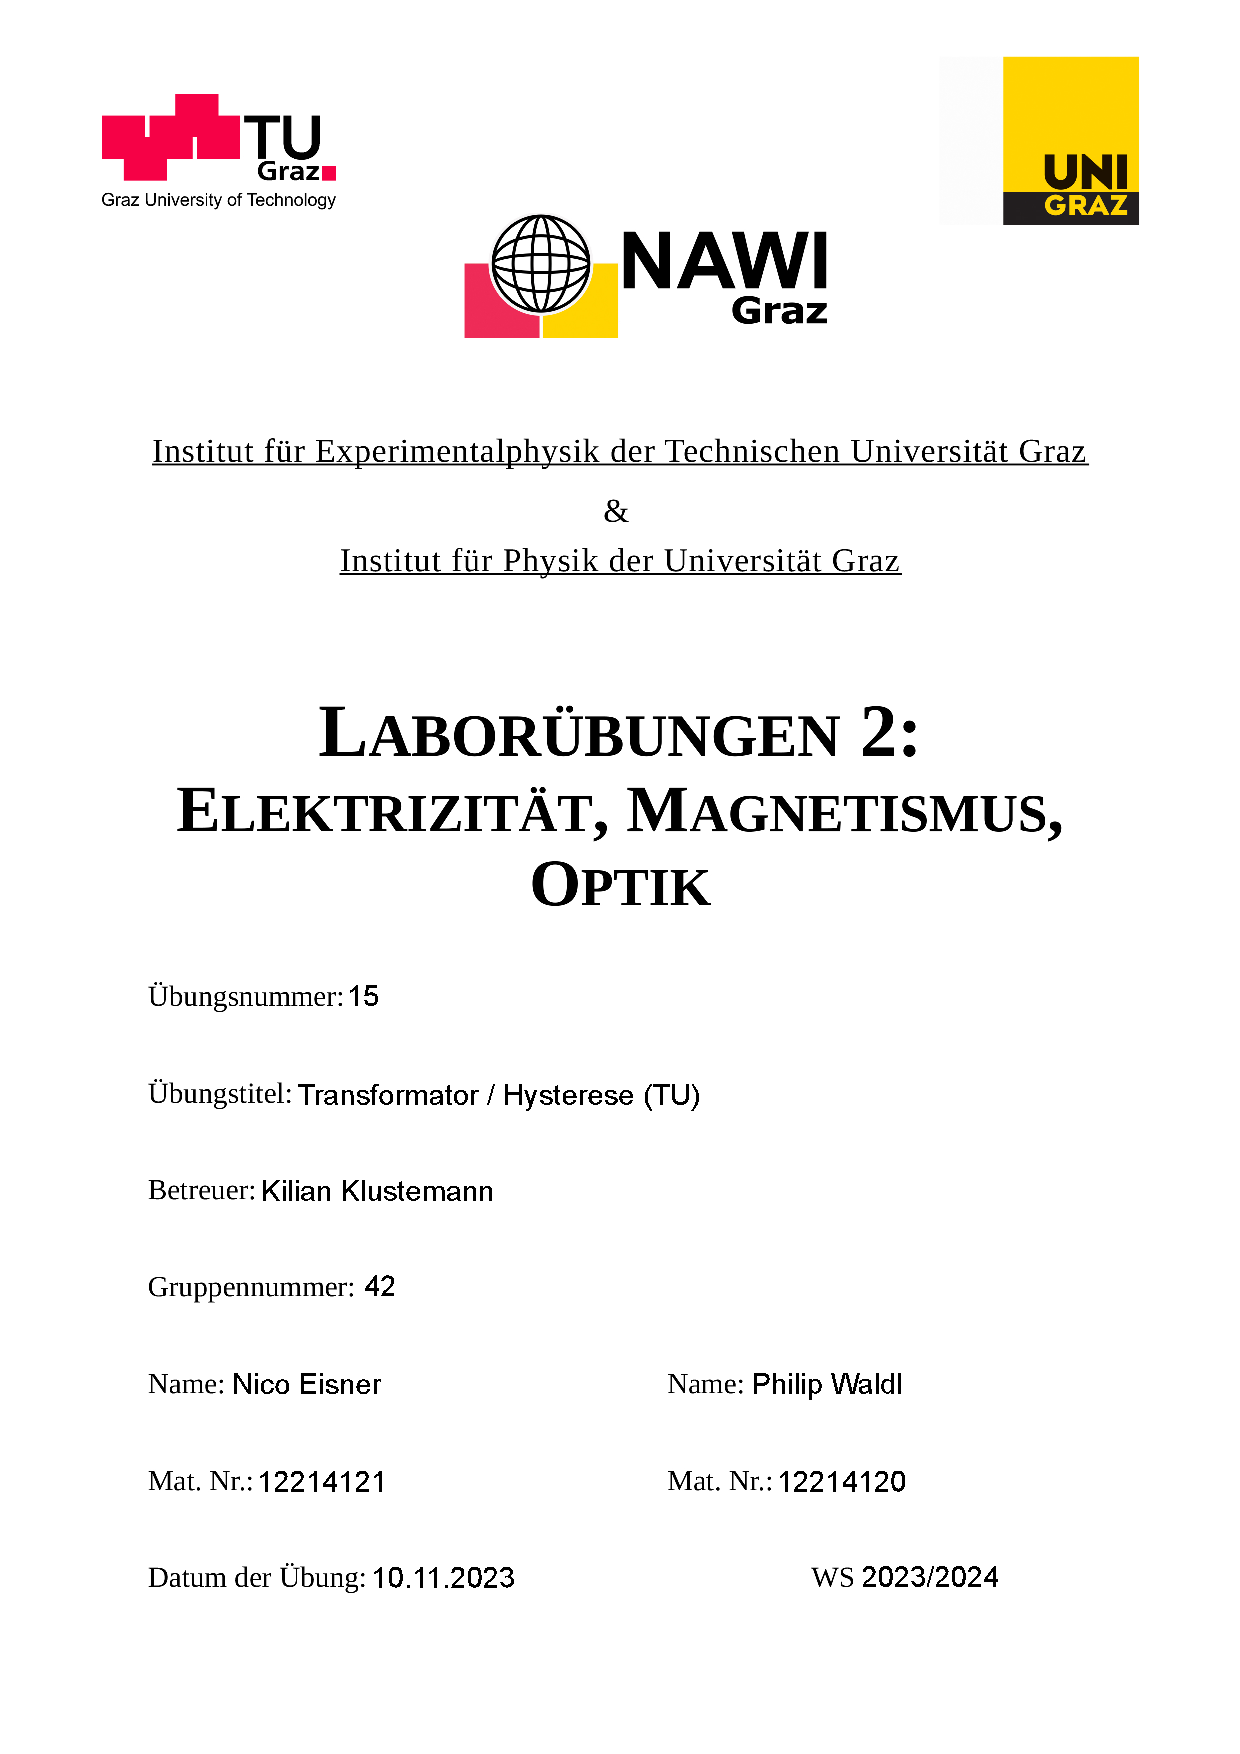
\includepdf[pages={1}]{../Deckblätter/Deckblatt_Transformator.pdf}

\tableofcontents
\newpage

\section{Aufgabenstellung} %jo beschreibn wos gmocht host ------------------------------
Der Versuch Transformator / Hysterese behandelt, wie aus dem Namen bereits hervorgeht, den Funktionsbereich des Transformators, in welchem in erster Linie die Umwandlung von elektsichen Spannungen hineinfällt.
Anhand von einer elektrischen Schaltung, welche im weiteren Verlauf des Experimentes immer wieder erweitert wird, soll die Rolle des Transformators veranschaulicht werden.
Zu erledigen war dabei folgender Versuchsauftrag:

\begin{itemize}
    \item Schaltung im Leerlauf
    \begin{itemize}
        \item Primärstrom $I_{1}$
        \item Primärspannung $U_{1}$
        \item Wirkleistung $P_{1}$
        \item Sekundärspannung $U_{2}$
        \item Sekundärstrom $I_{2}$
        \item Oszillographische Darstellung von Primärstrom und Sekundärspannung
    \end{itemize}
    \item Schaltung mit Ohm'scher Last sekundärseitig
    \begin{itemize}
        \item Primärstrom $I_{1}$
        \item Primärspannung $U_{1}$
        \item Wirkleistung $P_{1}$
        \item Sekundärspannung $U_{2}$
        \item Sekundärstrom $I_{2}$
        \item Oszillographische Darstellung von Primärstrom und Sekundärspannung
    \end{itemize}
    \item Schaltung mit Ohm'sch-induktiver Last (für ca. 20 Widerstandswerte)
    \begin{itemize}
        \item Primärstrom $I_{1}$
        \item Primärspannung $U_{1}$
        \item Wirkleistung $P_{1}$
        \item Sekundärspannung $U_{2}$
        \item Sekundärstrom $I_{2}$
        \item Oszillographische Darstellung der Sekundärspannung an der Stelle mit der größten Wirkleistung
    \end{itemize}
    \item \sout{Schaltung mit Ohm'sch-kapazitiver Last}
    \item Unsicherheitsberechnung für alle Punkte
\end{itemize}

\noindent
Alle Informationen und Methodiken wurden uns von der Technischen Universität bereitgestellt \cite{teachcenter1}. 


\section{Voraussetzungen \& Grundlagen} %Grundlagen erklären, Formeln mit erklärung

Wie im vorherigen Kapitel bereits eingeleitet dient ein Transformator dazu, von einer elektrischen Spannung auf eine andere zu transformieren. Im Aufbau sieht er dabei vereinfacht so aus:

\begin{figure}[H]
    \centering
    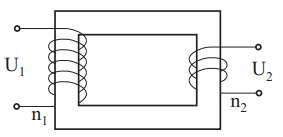
\includegraphics[width=0.5\linewidth]{nudes/GL-TrafoAufbau.png}
    \caption{Grundlegender Aufbau eines Transformators \cite{teachcenter1}}
    \label{fig:Aufbau Transformator}
\end{figure}

\noindent
Wie sich in Abbildung \ref{fig:Aufbau Transformator} erkennen lässt, besteht der Transformator aus zwei Spulen, welche über einen Eisenjoch miteinander verbunden sind. Die Umwandlung der Spannungen basiert auf dem Faraday'schen Gesetz

    \begin{equation}
        \label{eq:Faraday'sches Gesetz}
        \centerline{$U_{ind}=-N_{ind}\frac{d \phi}{dt}$}
    \end{equation}

\noindent
Wenn an der Primärspule eine Wechselspannung angelegt wird, wird ein sich änderndes (aufgrund der Richtungsänderung der Wechselspannung) Magnetfeld an der Primärspule (Eingangsspule) erzeugt. Durch dieses Magnetfeld wird an der Sekundärspule gemäß \ref{eq:Faraday'sches Gesetz} eine Ausgangsspannung induziert. 
Die resultierende Spannung ist dabei abhängig vom Wicklungsverhältnis der Spulen, was sich mit dem Ausdruck

\begin{equation}
    \label{eq:Verhältnis Wicklungen/Spannung}
    \centerline{$\frac{U2}{U1}=-\frac{n2}{n1}$}
\end{equation}

\noindent
beschreiben lässt. Der magnetische Fluss $\Phi$ setzt socj weiters in folgender Form zusammen:

\begin{equation}
    \label{eq:Magnetischer Fluss}
    \centerline{$\Phi = BA = \mu \mu_{0} HA = \mu \mu_{0} \frac{A}{l} nI$}
\end{equation}

\noindent
Sollte die Magnetisierungskurve $\Phi = \Phi(t)$ eine Hysterese, also eine verzögerte Entmagnetisierung von Ferromagnetischen Stoffen, aufweisen, so wird dem System Leistung entzogen und der Stromverlauf sieht wie folgt aus:

\begin{figure}[H]
    \centering
    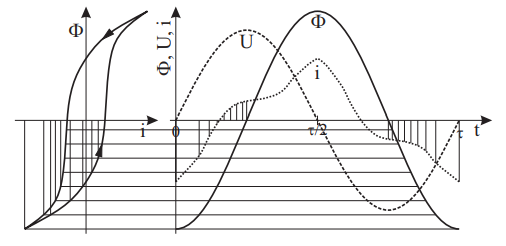
\includegraphics[width=0.5\linewidth]{nudes/GL-Hysterese.png}
    \caption{Magentischer Fluss mit Hysterese}
    \label{fig:Hystere}
\end{figure}

\noindent
Die Fläche innerhalb der in Abbildung \ref{fig:Hystere} gezeigten Hystereseschleife gibt Auskunft über die Hystereseverluste, welche gemeinsam mit den Wirbelstromverlusten die Eisenverluste am Trafo ergeben. \newline

\noindent
Außerdem werden für die Auswertung noch folgende Zusammenhänge benötigt:

\begin{equation}
    \label{eq:Scheinleistung}
    \centerline{$P_{S1} = U_{1}*I_{1}$ \\ $\Delta P_{S1} = \vert \frac{\partial P_{S1}}{\partial U_{1}} * \Delta U_{1} \vert + \vert \frac{\partial P_{S1}}{\partial I_{1}} * \Delta I_{1} \vert $}
\end{equation}

\begin{equation}
    \label{eq:Leistungsfaktor}
    \centerline{$cos(\Phi) = \frac{P_{1}}{S_{1}}$ \\ $\Delta cos(\Phi) = \vert \frac{\partial cos(\Phi)}{\partial P_{1}} * \Delta P_{1} \vert + \vert \frac{\partial cos(\Phi)}{\partial S_{1}} * \Delta S_{1} \vert $}
\end{equation}

\begin{equation}
    \label{eq:Verlustleistung}
    \centerline{$P_{V} = P_{1} - P_{2}$ \\ $\Delta P_{V} = \vert \frac{\partial P_{V}}{\partial P_{1}} * \Delta P_{1} \vert + \vert \frac{\partial P_{V}}{\partial P_{2}} * \Delta P_{2} \vert $}
\end{equation}

\begin{equation}
    \label{eq:Blindleistung}
    \centerline{$P_{Q1} = \sqrt{S_{1}^2 - P_{1}^2}$ \\ $\Delta P_{Q1} = \vert \frac{\partial P_{Q1}}{\partial S_{1}} * \Delta S_{1} \vert + \vert \frac{\partial P_{Q1}}{\partial P_{1}} * \Delta P_{1} \vert $}
\end{equation}

\begin{equation}
    \label{eq:Wirkleistung}
    \centerline{$P_{W2} = U_{2}*I_{2}$ \\ $\Delta P_{S1} = \vert \frac{\partial P_{W2}}{\partial U_{2}} * \Delta U_{2} \vert + \vert \frac{\partial P_{W2}}{\partial I_{2}} * \Delta I_{2} \vert $}
\end{equation}

\begin{equation}
    \label{eq:Wirkungsgrad}
    \centerline{$\eta = \frac{P_{2}}{S_{1}}$ \\ $\Delta \eta = \vert \frac{\partial \eta}{\partial P_{2}} * \Delta P_{2} \vert + \vert \frac{\partial \eta}{\partial S_{1}} * \Delta S_{1} \vert $}
\end{equation}

\begin{equation}
    \label{eq:OhmschesGesetz}
    \centerline{$R = \frac{U}{I}$ \\ $\Delta R = \vert \frac{\partial R}{\partial U} * \Delta U \vert + \vert \frac{\partial R}{\partial I} * \Delta I \vert $}
\end{equation}


\section{Versuchsanordnung} %mit skizze kurz beschreiben ------------------------------

Das Herzstück des Versuches ist natürlich der Trafo, wobei bei diesem Experiment gleich zwei zum Einsatz kommen. Der gesamte Versuch basiert auf einer Grundschaltung, welche mit jedem Aufgabenpunkt ein wenig erweitert wird.

    \begin{figure}[H]
        \centering
        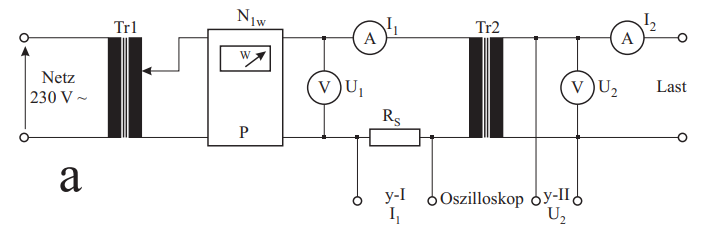
\includegraphics[width=0.6\linewidth, angle=0]{nudes/Versuchsaufbau a.png}
        \caption{Aufbau der Grundschaltung}
        \label{fig:AufbauDerGrundschaltung}
    \end{figure}

\noindent
In der Realität sieht der Aufbau wie folgt aus:

\begin{figure}[H]
    \centering
    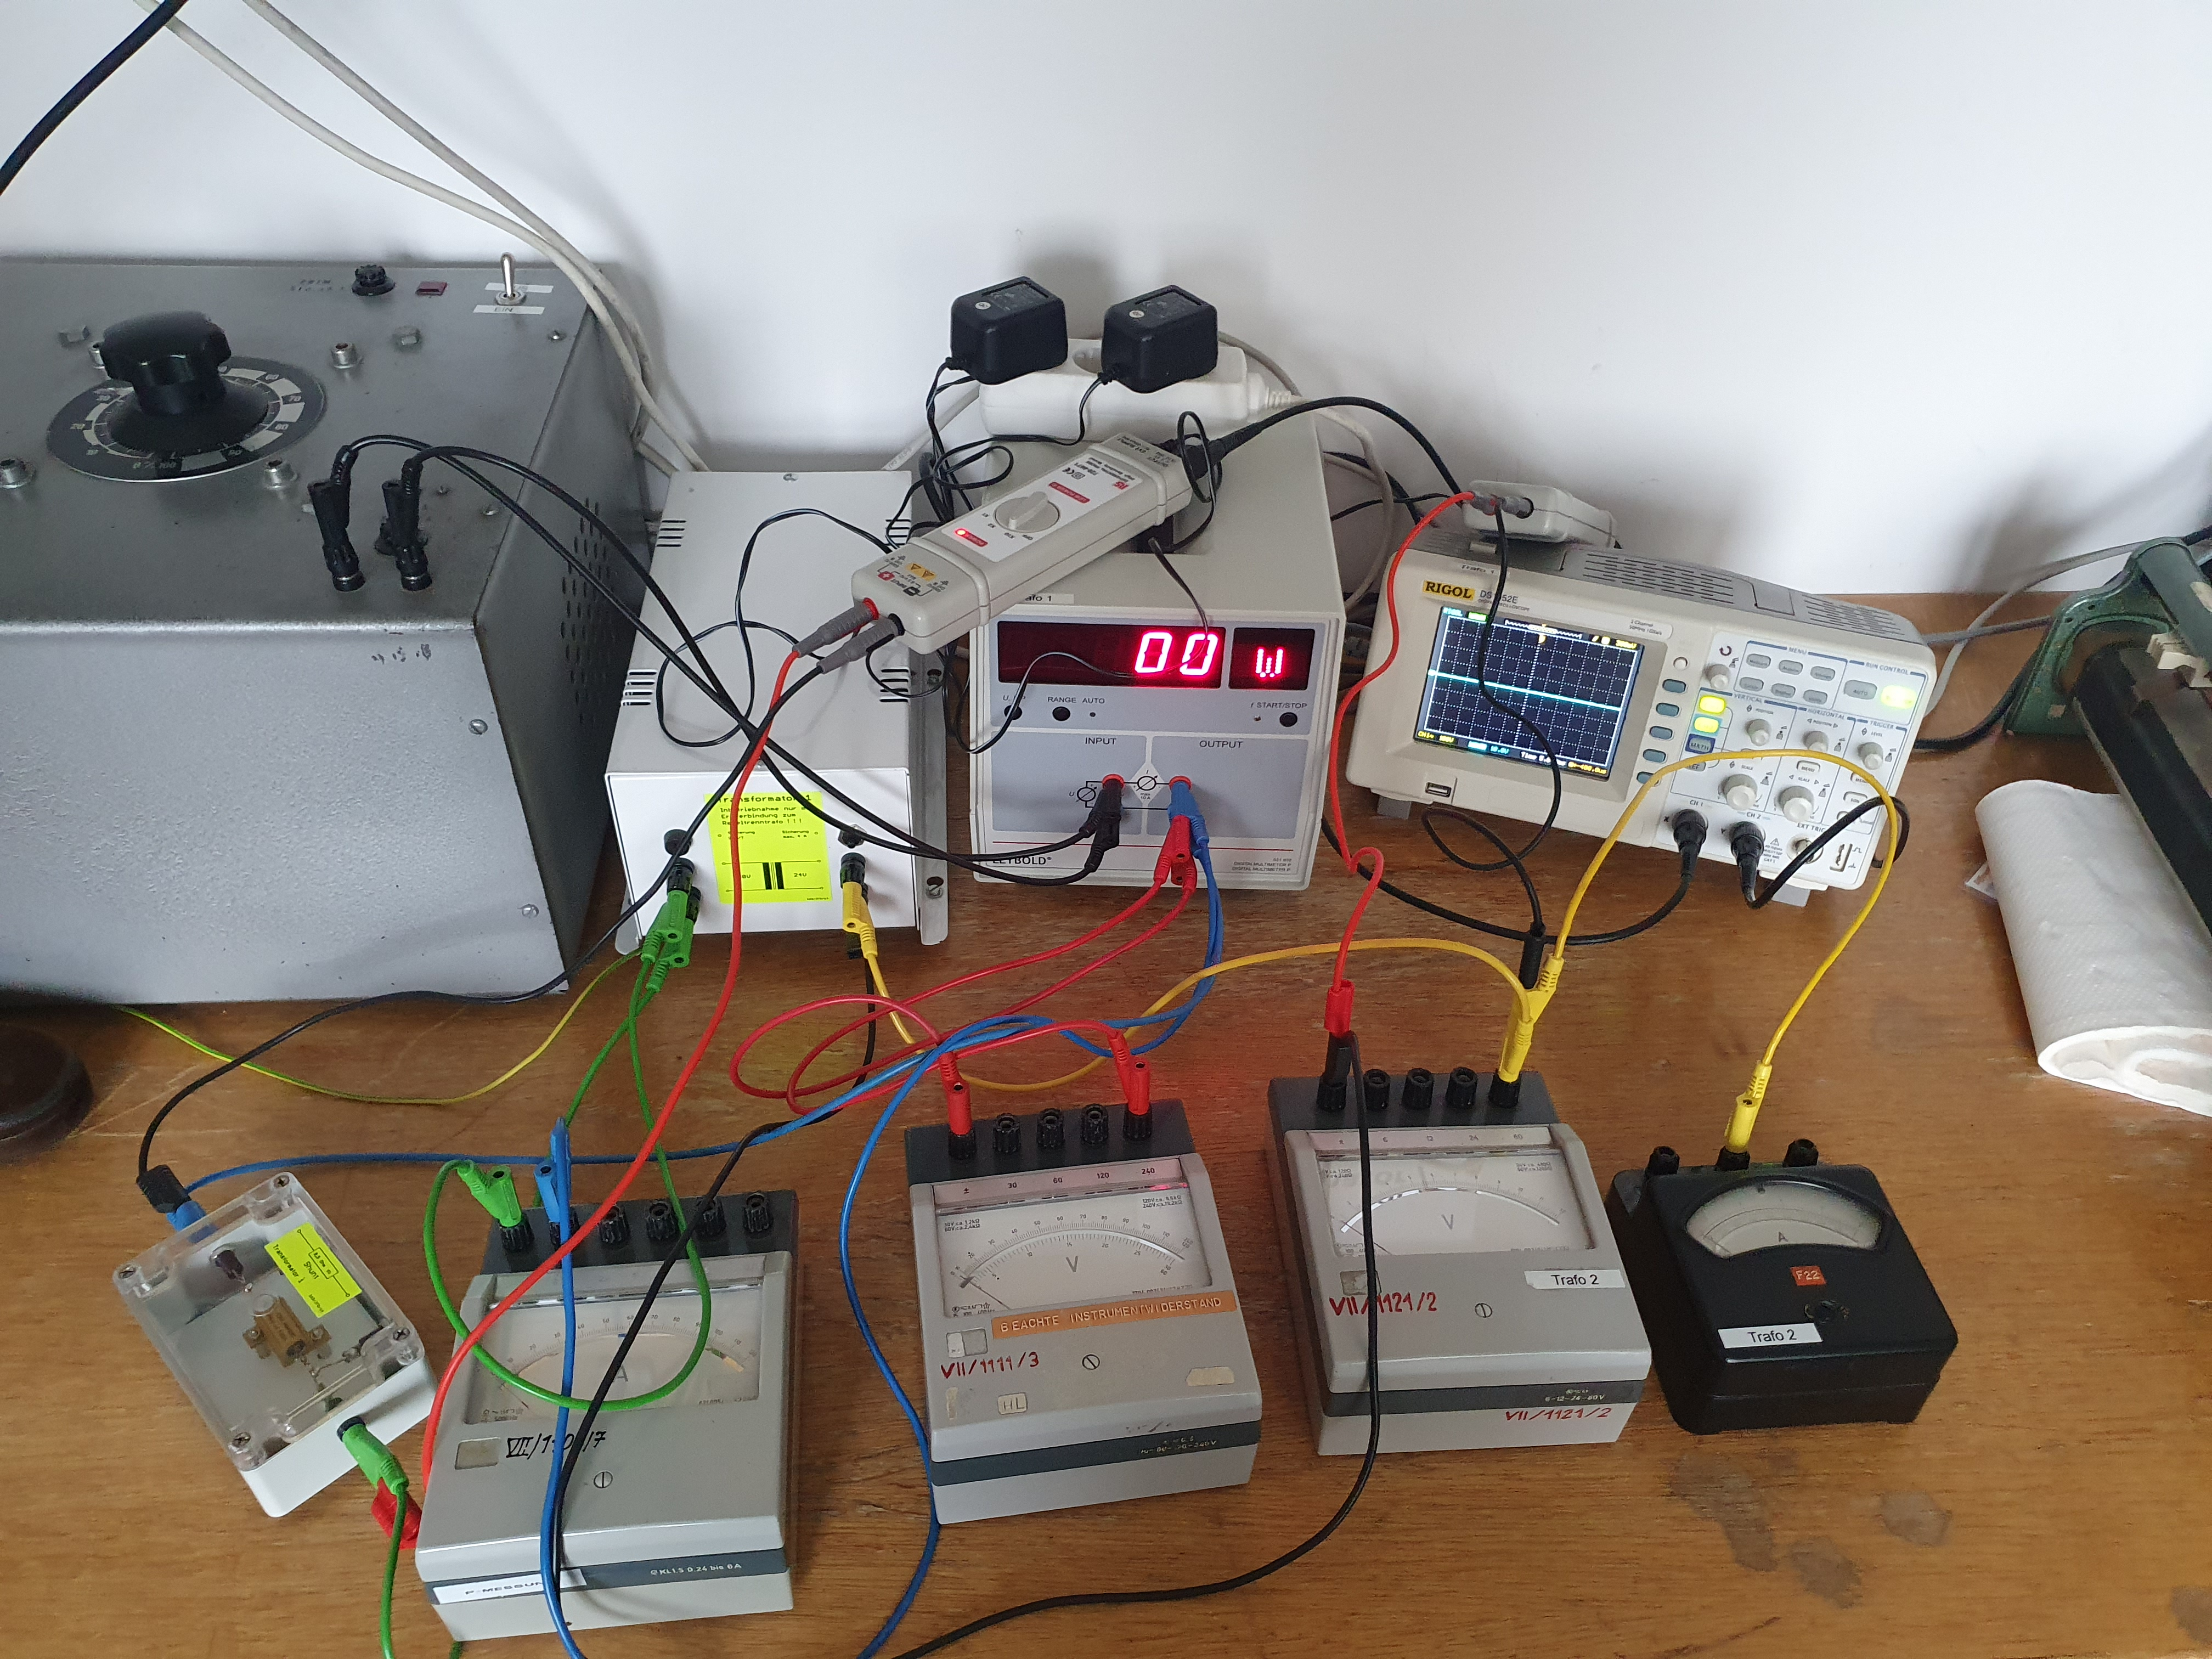
\includegraphics[width=0.6\linewidth, angle=0]{nudes/Aufbau a.png}
    \caption{Realer Aufbau der Grundschaltung}
    \label{fig:RealerAufbauDerGrundschaltung}
\end{figure}

\noindent
Im weiteren Verlauf des Experimentes wurde die Schaltung nicht wie in Abbildung \ref{fig:RealerAufbauDerGrundschaltung} im Leerlauf, sondern mit einem Lastwiderstand $R_{L}$ betrieben. Dadurch konnte nun auch ein Verbraucherstrom $I_{2}$ gemessen werden. Aufgebaut sieht der Versuch nun so aus:

\begin{figure}[H]
    \centering
    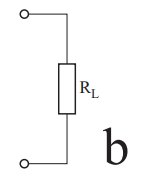
\includegraphics[width=0.2\linewidth, angle=0]{nudes/Versuchsaufbau b.png}
    \caption{Hinzugefügter Lastwiderstand}
    \label{fig:AufbauB}
\end{figure}

\begin{figure}[H]
    \centering
    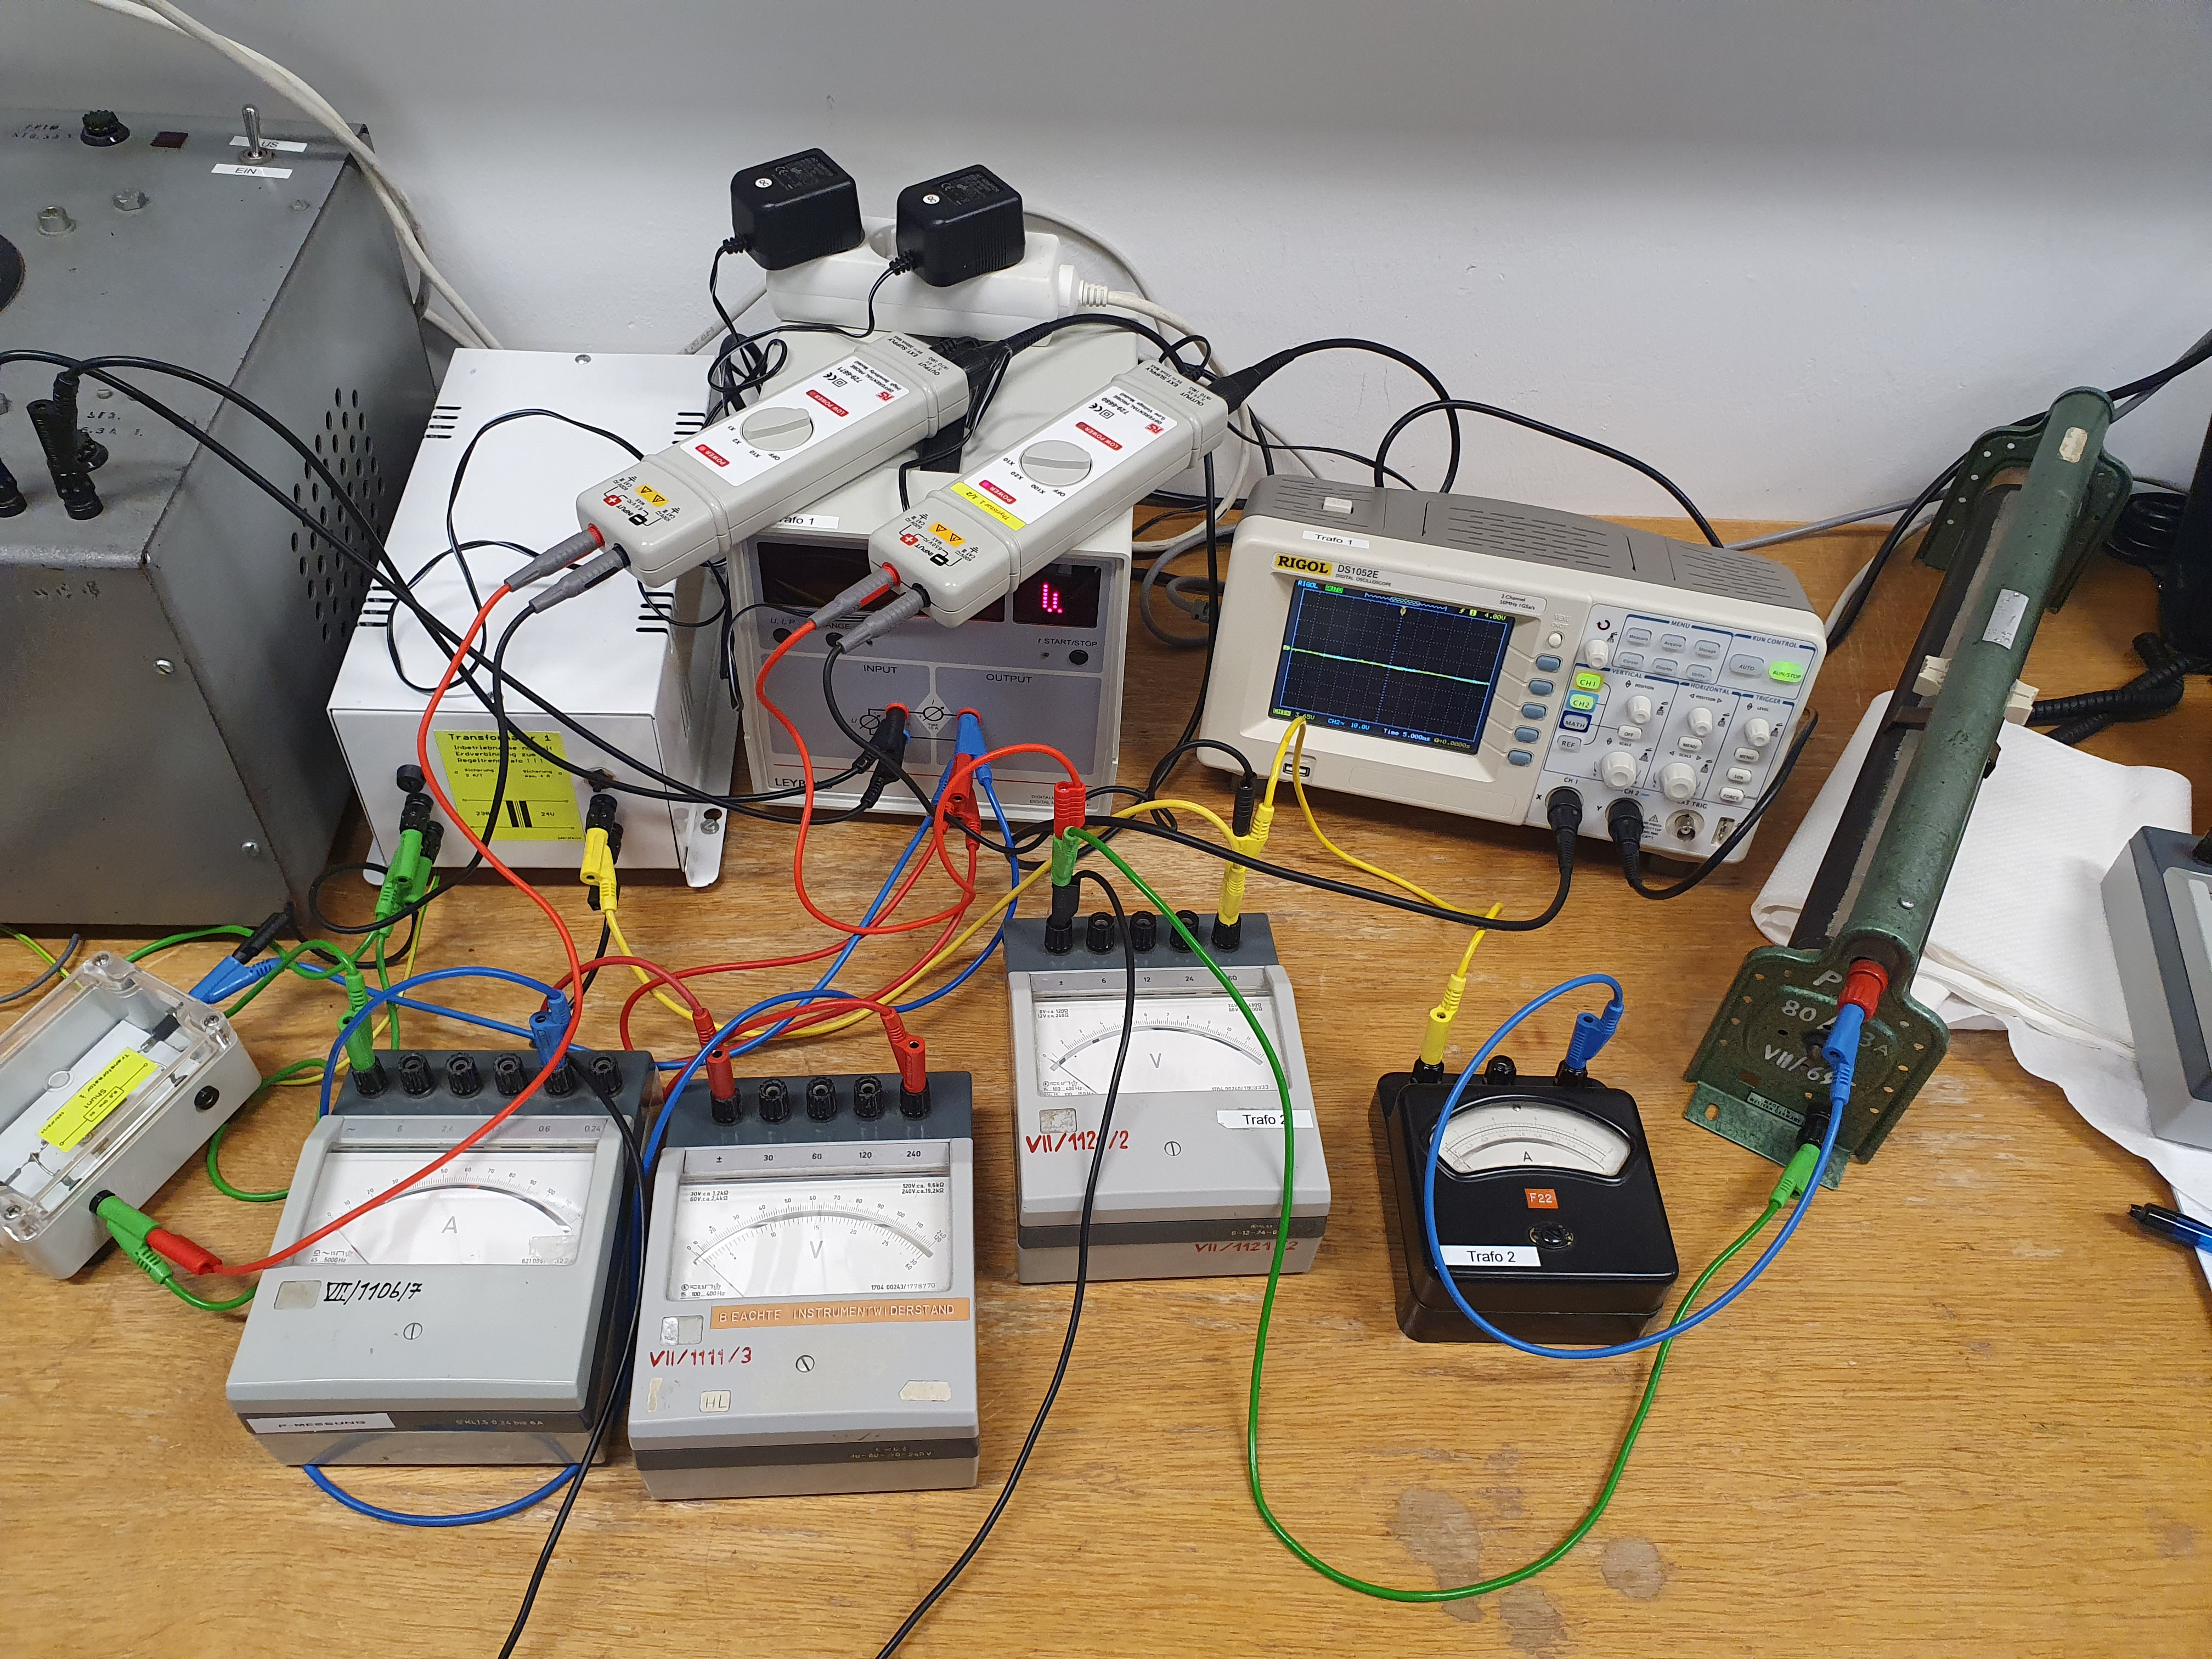
\includegraphics[width=0.6\linewidth, angle=0]{nudes/Aufbau b.png}
    \caption{Realer Aufbau mit Lastwiderstand}
    \label{fig:RealerAufbauB}
\end{figure}

\noindent
Für die letzte Erweiterung der Grundschaltung wurde nun noch eine Spule seriell an das Potentiometer angeschlossen. Weiters war nun ein weiteres Voltmeter zur Bestimmung der Spannung $U_{R}$, welche später für die Berechnung der Leistung $P_{2}$ noch benötigt wird.

\begin{figure}[H]
    \centering
    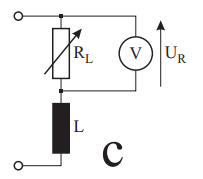
\includegraphics[width=0.2\linewidth, angle=0]{nudes/Versuchsaufbau c.png}
    \caption{Potentiometer und Spule als zusätzliche Verbraucher}
    \label{fig:AufbauC}
\end{figure}

\begin{figure}[H]
    \centering
    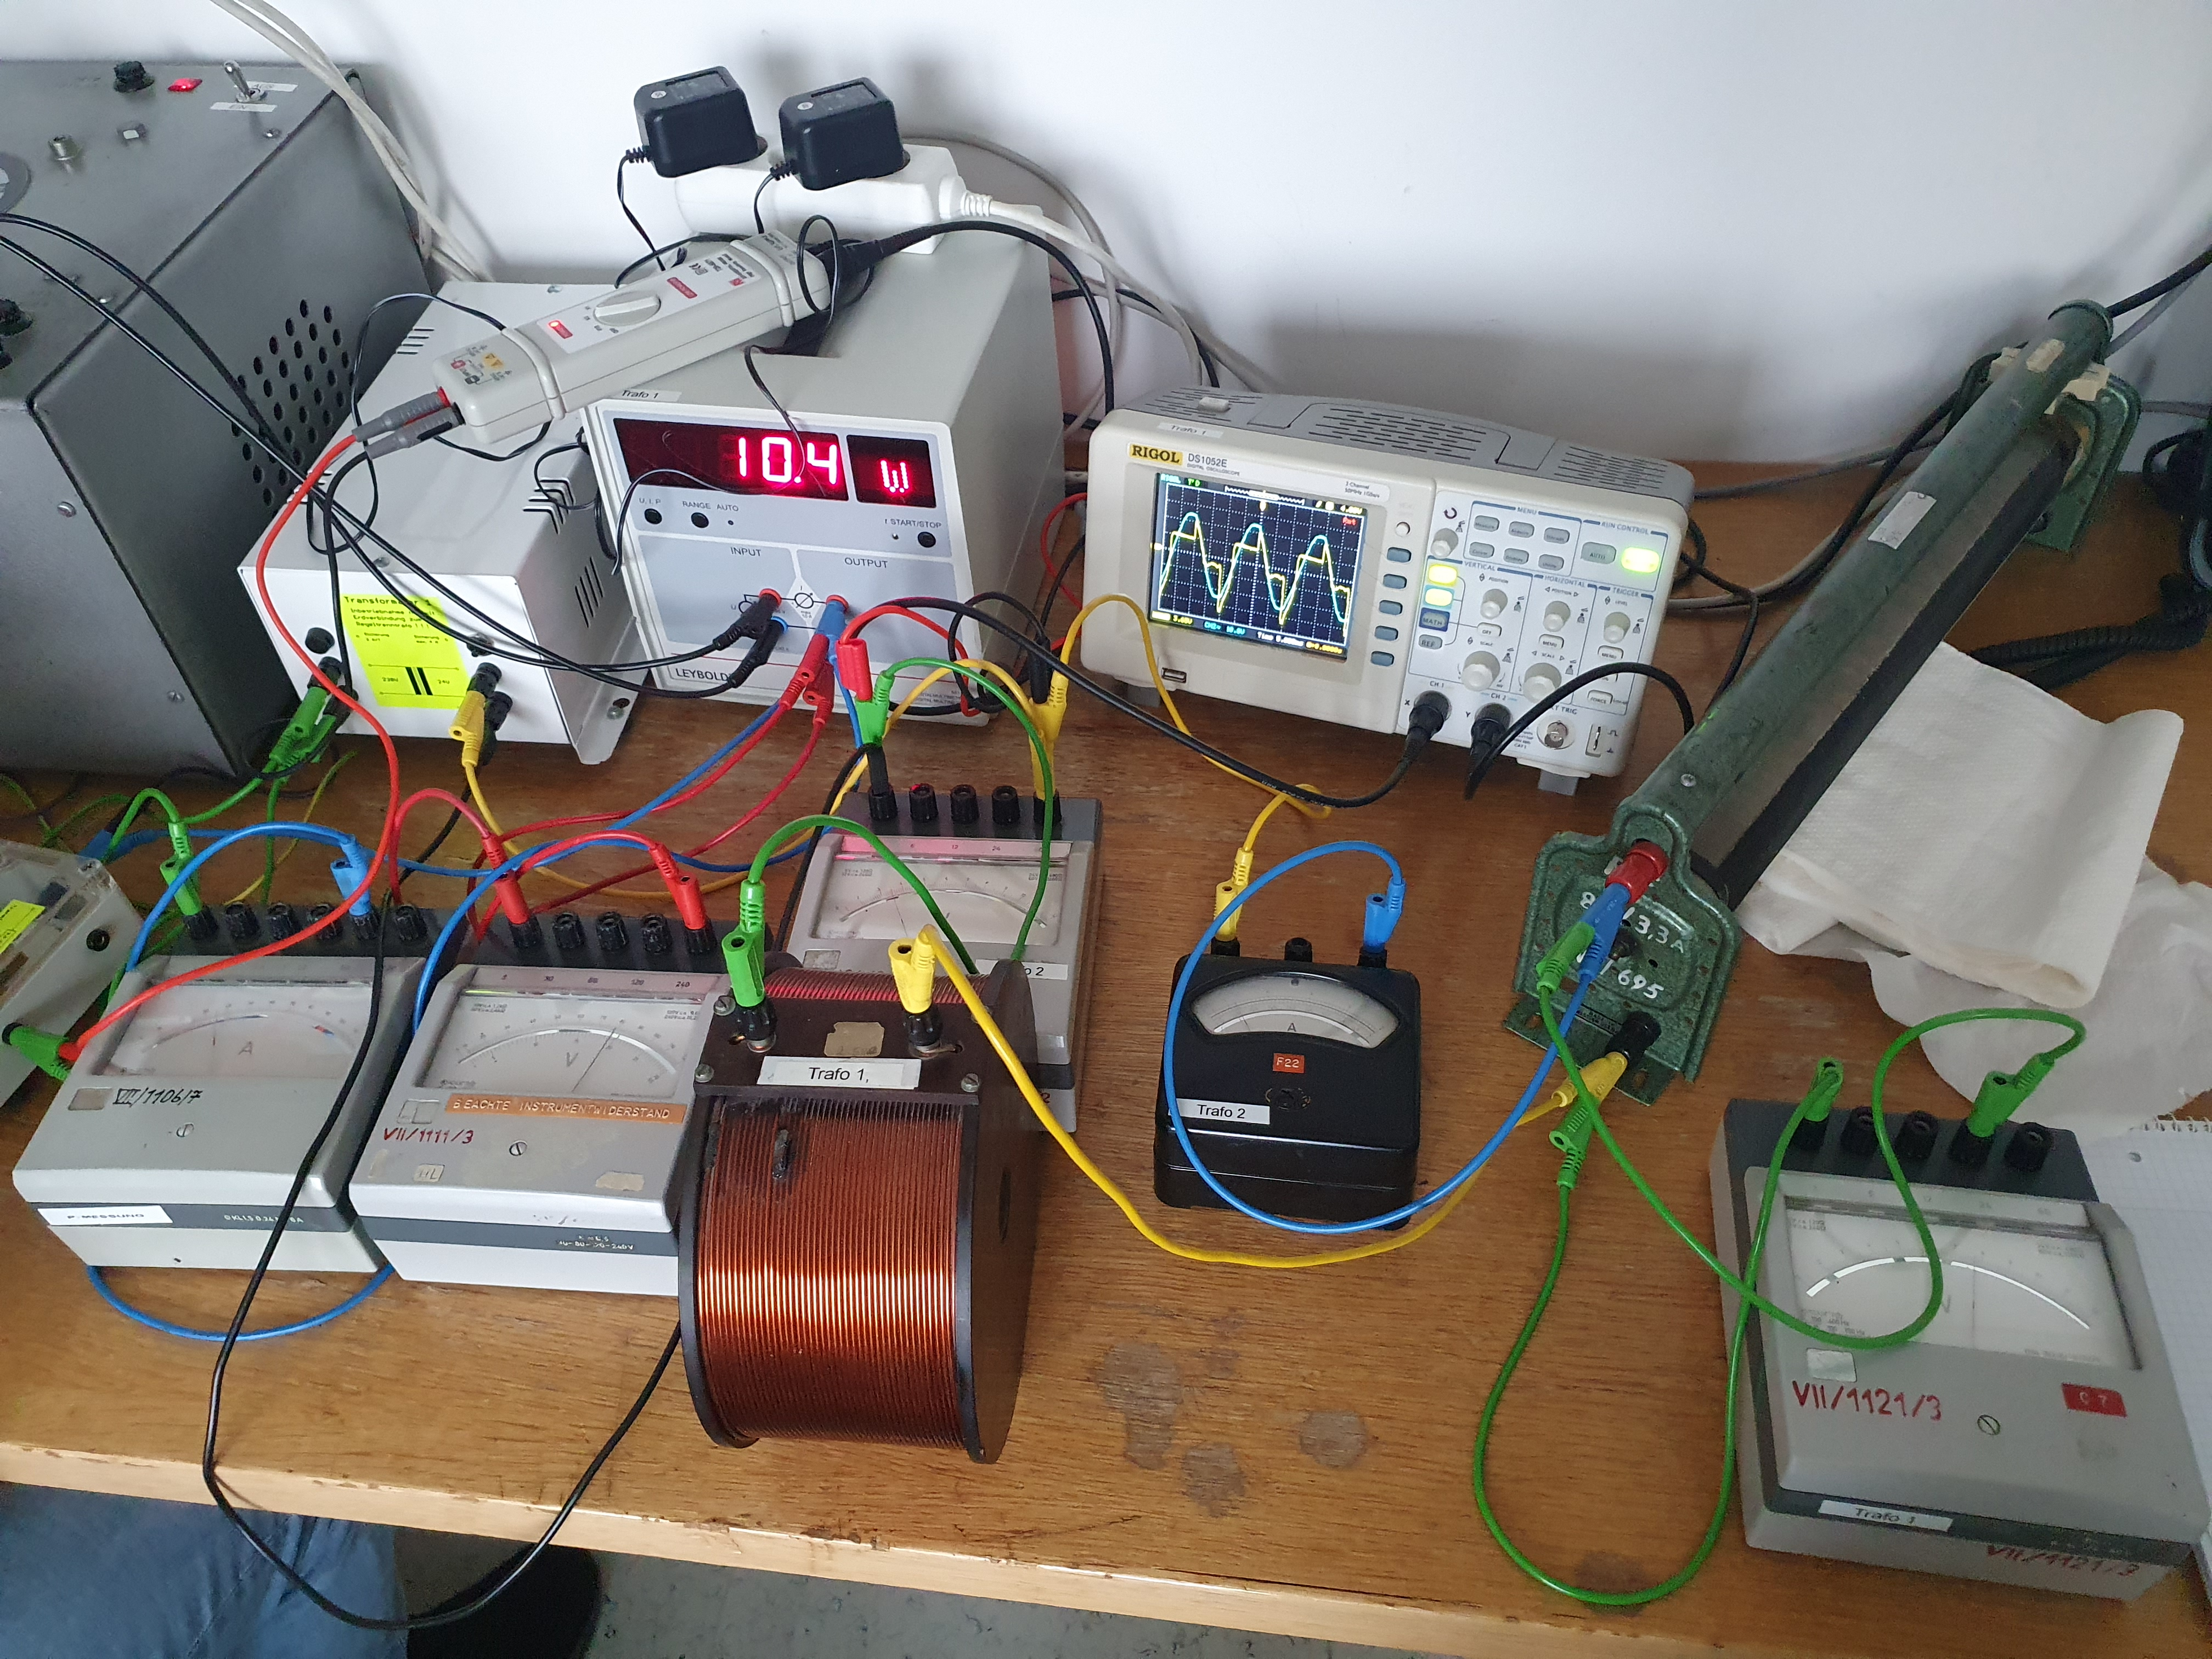
\includegraphics[width=0.6\linewidth, angle=0]{nudes/Aufbau c.png}
    \caption{Realer Aufbau mit Potentiometer und Spule}
    \label{fig:RealerAufbauC}
\end{figure}



\section{Geräteliste} %jo holt a listn ------------------------------

    \begin{table}[H]
        \centering
        \caption{Im Versuch verwendete Geräte und Utensilien.}
        \label{tab:geraete}
        \begin{tabular}{| l | l | l | l |}
            \hline
            Gerät & Gerätenummer  & Unsicherheit \\
            Oszilloskop & {n.a} & {n.a} \\
            Trafo Tr1 & {n.a} & {n.a} \\
            Trafo Tr2 & {n.a} & {n.a} \\
            Multimeter P & {n.a} & $\pm 0.01 W$ \cite{leybold}\\
            Potentiometer & {n.a} & {n.a} \\
            Shunt & {n.a} & {n.a} \\
            Voltmeter U1 & {n.a} & $\pm 0.5\%$ + 2 digit \\
            Voltmeter U2 & {n.a} & $\pm 0.5\%$ + 2 digit \\
            Voltmeter UR & {n.a} & $\pm 0.5\%$ + 2 digit \\
            Amperemeter I1 & {n.a} & $\pm 1.5\%$ + 2 digit \\
            Amperemeter I2 & {n.a} & $\pm 0.5\%$ + 2 digit \\
            Spule & {n.a} & {n.a} \\
            \hline
        \end{tabular}
    \end{table}


\section{Versuchsdurchführung \& Messergebnisse} %nachvollziehbar und klar dargestellt ------------------------------

\subsection{Leerlauf}

Zu Beginn des ersten Teiles des Versuches wurde die grundlegende Schaltung laut \ref{fig:AufbauDerGrundschaltung} aufgebaut und vom Betreuer kontrolliert.
Wie in der Aufgabenstellung erwähnt befindet sich hier noch kein Lastwiderstand im System, weshalb kein Sekundärstrom $I_{2}$ fließt. Sobald der Aufbau abgeschlossen war, wurde der Stromkreis durch einschalten des Trafo 1 geschlossen und es konnten alle benötigten Werte von den Messgeräten abgelesen werden.
Hierbei galt noch zu Beachten, dass die angezeigten Werte der alten Volt- und Amperemeter nicht einfach zu übernehmen waren. Der Maximalwert der Skala war gleich dem Wert des jeweiligen Anschlusses (in Abbildung \ref{fig:MessgerätWerte} grün markiert):

\begin{figure}[H]
    \centering
    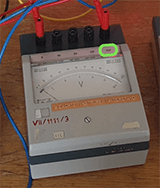
\includegraphics[width=0.4\linewidth, angle=0]{nudes/VoltmeterBeschriftung.png}
    \caption{Messgeräte Werte}
    \label{fig:MessgerätWerte}
\end{figure}

\noindent
Somit ergibt sich als Beispiel für dieses Voltmeter aus Abbildung \ref{fig:MessgerätWerte} ein Maximalwert von 240V. Wenn der Zeiger also beispielsweiße bei der Hälfte wäre, dann hätte die Spannung nicht wie beschriftet 60V, sondern 120V ($\frac{240}{2}$). Diese Umrechnung wurde für die gemessenen Werte bei den jeweiligen Messgeräten bereits durchgeführt und nur die tatsächlichen Zahlen in die Tabelle eingetragen.

\begin{table}[H]
    \centering
    \caption{Messwerte Leerlauf}
    \label{tab:messwerteLeerlauf}
    \resizebox{\columnwidth}{!}{\begin{tabular}{|l|l|l|l|l|}
        \hline
        Primärstrom $I_{1}$ / A  & Primärspannung $U_{1}$ / V & Sekundärspannung $U_{2}$ / V & Wirkleistung $P_{1}$ / W \\
        \hline
        0.170 $\pm$ 0.011 & 160.0 $\pm$ 1.4 & 17.3 $\pm$ 0.5 & 6.90 $\pm$ 0.01 \\
        \hline
    \end{tabular}}
\end{table}

\noindent
Die oszillographische Darstellung des Primärstromes und der Sekundärspannung werden in folgender Abbildung grafisch dargestellt.

\begin{figure}[H]
    \centering
    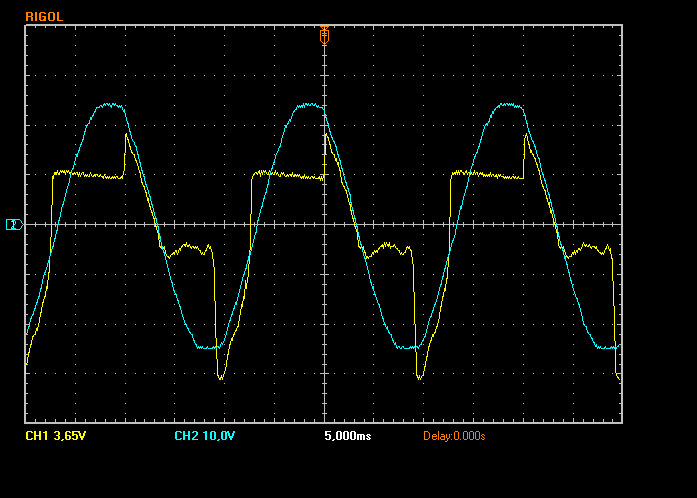
\includegraphics[width=0.6\linewidth, angle=0]{nudes/A1 Oszi.jpg}
    \caption{Oszillographische Darstellung Primärstromes und Sekundärspannung}
    \label{fig:OszilloskopA}
\end{figure}


\subsection{Ohm'sche Last sekundärseitig}

Im nächsten Aufgabenteil wurde nun die Grundschaltung mit dem Potentiometer (Abbildung \ref{fig:AufbauB}) erweitert. Nachdem die Schaltung wieder kontrolliert wurde, konnten die Werte mit dem selben System wie im vorherigen Punkt abgelesen und umgerechnet werden.
Jedoch konnte nun auch der Sekundärstrom $I_{2}$ bestimmt werden. Der Schieberegler des Potentiometers wurde dabei ungefähr auf die Mitte geschoben, was einem Widerstand von etwa 42 Ohm entspricht.

\begin{table}[H]
    \centering
    \caption{Messwerte Ohm'sche Last}
    \label{tab:messwerteOhm}
    \resizebox{\columnwidth}{!}{\begin{tabular}{|l|l|l|l|l|}
        \hline
        P. Strom $I_{1}$ / A  & P. Spannung $U_{1}$ / V & Strom $I_{2}$ / A & S. Spannung $U_{2}$ / V & Wirkleistung $P_{1}$ / W \\
        \hline
        0.195 $\pm$ 0.011 & 160.0 $\pm$ 1.4 & 0.640 $\pm$ 0.007 & 17.0 $\pm$ 0.5 & 17.90 $\pm$ 0.01 \\
        \hline
    \end{tabular}}
\end{table}

\noindent
Die grafische Darstellung des Primärstromes und der Sekundärspannung mittels Oszilloskop sind in folgendem Bild ersichtlich.

\begin{figure}[H]
    \centering
    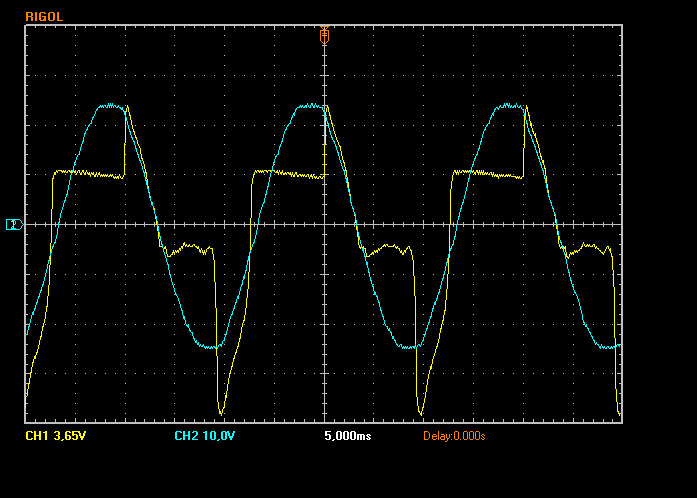
\includegraphics[width=0.6\linewidth, angle=0]{nudes/A2 Oszi.jpg}
    \caption{Oszillographische Darstellung Primärstromes und Sekundärspannung}
    \label{fig:OszilloskopB}
\end{figure}


\subsection{Ohm'sche-induktive Last}

Beim dritten Abschnitt des Versuches wird die Schaltung wieder etwas erweitert. Nun kommt zum Potentiometer noch eine Spule L (Abbildung \ref{fig:AufbauC}) hinzu.
Außerdem wird nun kein fester Widerstand am Potentiometer eingestellt, sondern dieser wird Schrittweiße verschoben, sodass 22 Messungen entstehen. Weiters wurde zur späteren Bestimmung der Wirkleistung $P_{2}$ die Spannung $U_{R}$ am Potentiometer gemessen.

\begin{table}[H]
    \centering
    \caption{Messwerte Ohm'sche und induktive Last}
    \label{tab:messwerteOhmInduktiv}
    \resizebox{\columnwidth}{!}{\begin{tabular}{|l|l|l|l|l|l|l|}
        \hline
        Nr. & $I_{1}$ $\pm$ 0.011 / A & $U_{1}$ $\pm$ 1.4 / V & $I_{2}$ $\pm$ 0.007 / A & $U_{2}$ $\pm$ 0.5 / V & $P_{1}$ $\pm$ 0.01 / W & $U_{R}$ $\pm$ 0.14 / V \\
        \hline
        1  & 0.180 & 160.0 & 0.220 & 17.0 & 10.40 & 15.20 \\
        2  & 0.183 & 160.0 & 0.220 & 17.0 & 10.50 & 15.20 \\
        3  & 0.185 & 160.0 & 0.230 & 17.0 & 10.60 & 15.00 \\
        4  & 0.185 & 160.0 & 0.240 & 17.0 & 10.60 & 15.00 \\
        5  & 0.189 & 160.0 & 0.240 & 17.0 & 10.70 & 14.90 \\
        6  & 0.189 & 160.0 & 0.250 & 17.0 & 10.80 & 14.80 \\
        7  & 0.189 & 160.0 & 0.250 & 17.0 & 10.80 & 14.60 \\
        8  & 0.189 & 160.0 & 0.260 & 17.0 & 10.90 & 14.40 \\
        9  & 0.188 & 160.0 & 0.270 & 17.0 & 11.00 & 14.30 \\
        10 & 0.190 & 160.0 & 0.280 & 17.0 & 11.10 & 14.10 \\
        11 & 0.190 & 160.0 & 0.290 & 17.0 & 11.30 & 13.80 \\
        12 & 0.190 & 160.0 & 0.300 & 17.0 & 11.40 & 13.60 \\
        13 & 0.193 & 160.0 & 0.320 & 17.0 & 11.50 & 13.20 \\
        14 & 0.195 & 160.0 & 0.330 & 17.0 & 11.50 & 13.00 \\
        15 & 0.195 & 160.0 & 0.340 & 17.0 & 11.60 & 12.60 \\
        16 & 0.198 & 160.0 & 0.360 & 17.3 & 11.70 & 12.20 \\
        17 & 0.200 & 160.0 & 0.380 & 17.0 & 11.80 & 11.60 \\
        18 & 0.203 & 160.0 & 0.400 & 17.0 & 11.80 & 11.00 \\
        19 & 0.205 & 160.0 & 0.420 & 17.0 & 11.70 & 10.40 \\
        20 & 0.205 & 160.0 & 0.430 & 17.0 & 11.80 & 10.00 \\
        21 & 0.210 & 160.0 & 0.450 & 17.0 & 11.70 &  9.30 \\
        22 & 0.215 & 160.0 & 0.480 & 17.0 & 11.40 &  8.00 \\
        \hline
    \end{tabular}}
\end{table}



\section{Auswertung und Unsicherheitsanalyse} %Nicht nur zahlen angeben ------------------------------

In der Auswertung werden zur erhöhten Genauigkeit durchgehend ungerundete Werte bis zu den Endergebnissen verwendet und nur zur Darstellung gerundet. \\
Zur Berechnung der Unsicherheiten wird, wenn nicht anders angegeben, die Größtunsicherheitsmethode verwendet.

\subsection{Leerlauf}

Mittels Formeln \ref{eq:Scheinleistung}, \ref{eq:Leistungsfaktor} und \ref{eq:Blindleistung} werden nun gemeinsam mit den gemessenen Werten aus Tabelle \ref{tab:messwerteLeerlauf} die Scheinleistung $P_{S1}$, die Blindleistung $P_{Q1}$ und der Leistungsfaktor $cos(\Phi)$ berechnet.

\begin{table}[H]
    \centering
    \caption{Berechnungen Leerlauf}
    \label{tab:BerechnungenLeerlauf}
    \begin{tabular}{| l | l | l |}
        \hline
        $P_{S1}$ / W & $P_{Q1}$ / W & $cos(\Phi)$ / \\
        \hline
        27 $\pm$ 2 & 26 $\pm$ 3 & 0.26 $\pm$ 0.02 \\
        \hline
    \end{tabular}
\end{table}


\subsection{Ohm'sche Last sekundärseitig}

Auch hier sollen mit den Formeln \ref{eq:Scheinleistung}, \ref{eq:Leistungsfaktor}, \ref{eq:Blindleistung}, \ref{eq:Verlustleistung}, \ref{eq:Wirkleistung} und \ref{eq:Wirkungsgrad} werden nun gemeinsam mit den gemessenen Werten aus Tabelle \ref{tab:messwerteOhm} die Scheinleistung $P_{S1}$, die Blindleistung $P_{Q1}$, der Leistungsfaktor $cos(\Phi)$, die Verlustleistung $P_{V}$, die sekundärseitige Wirkleistung $P_{2}$ und der Wirkungsgrad $\eta$ berechnet.

\begin{table}[H]
    \centering
    \caption{Berechnungen Ohm}
    \label{tab:BerechnungenOhm}
    \begin{tabular}{| l | l | l | l | l | l |}
        \hline
        $P_{S1}$ / W & $P_{Q1}$ / W & $cos(\Phi)$ / & $P_{V}$ / W & $P_{2}$ / W & $\eta$ / \\
        \hline
        31.2 $\pm$ 2.1 & 25.5545 $\pm$ 3 & 0.58 $\pm$ 0.04 & 7.1 $\pm$ 0.6 & 10.9 $\pm$ 0.5 & 0.40 $\pm$ 0.04 \\
        \hline
    \end{tabular}
\end{table}


\subsection{Ohm'sche-induktive Last}

Für den letzten Aufgabenpunkt soll nun ein Leistung-Lastwiderstand-Diagramm erstellt werden. Hierzu wird mittels Formel \ref{eq:Wirkleistung} und den gemessenen Werten zu jedem Widerstandswert aus Tabelle \ref{tab:messwerteOhmInduktiv} die Leistung an den jeweiligen Potentiometerpositionen ermittelt.
Außerdem wurde mittels Ohm'schen Gesetz \ref{eq:OhmschesGesetz} der eingestellte Widerstand am Potentiometer berechnet.

\begin{table}[H]
    \centering
    \caption{Berechnete Werte für $R_{Pot}$ und $P_{2}$}
    \label{tab:berechnungenRPotP2}
    \begin{tabular}{| l | l | l |}
        \hline
        Nr.  & $R_{Pot}$ / $\Omega$ & $P_{2}$ / W \\
        \hline
        1  & 69 $\pm$ 3 & 3.35 $\pm$ 0.14 \\
        2  & 69 $\pm$ 3 & 3.35 $\pm$ 0.14 \\
        3  & 65 $\pm$ 3 & 3.45 $\pm$ 0.14 \\
        4  & 62 $\pm$ 3 & 3.60 $\pm$ 0.14 \\
        5  & 62 $\pm$ 3 & 3.58 $\pm$ 0.14 \\
        6  & 59 $\pm$ 3 & 3.70 $\pm$ 0.14 \\
        7  & 58 $\pm$ 3 & 3.65 $\pm$ 0.14 \\
        8  & 55 $\pm$ 3 & 3.75 $\pm$ 0.14 \\
        9  & 52.9 $\pm$ 1.9 & 3.87 $\pm$ 0.14 \\
        10 & 50.4 $\pm$ 1.8 & 3.95 $\pm$ 0.14 \\
        11 & 47.6 $\pm$ 1.7 & 4.01 $\pm$ 0.14 \\
        12 & 45.4 $\pm$ 1.6 & 4.08 $\pm$ 0.14 \\
        13 & 41.3 $\pm$ 1.4 & 4.23 $\pm$ 0.14 \\
        14 & 39.4 $\pm$ 1.3 & 4.29 $\pm$ 0.14 \\
        15 & 37.1 $\pm$ 1.2 & 4.29 $\pm$ 0.14 \\
        16 & 33.9 $\pm$ 1.1 & 4.40 $\pm$ 0.14 \\
        \textbf{17} & \textbf{30.6 $\pm$ 1.0} & \textbf{4.41 $\pm$ 0.14} \\
        18 & 27.5 $\pm$ 0.9 & 4.40 $\pm$ 0.14 \\
        19 & 24.8 $\pm$ 0.8 & 4.37 $\pm$ 0.14 \\
        20 & 23.3 $\pm$ 0.8 & 4.30 $\pm$ 0.14 \\
        21 & 20.7 $\pm$ 0.7 & 4.19 $\pm$ 0.13 \\
        22 & 16.7 $\pm$ 0.6 & 3.84 $\pm$ 0.13 \\
        \hline
    \end{tabular}
\end{table}

\noindent
Die fett markierte Zeile ist jene mit der höchsten Leistung. Sie stellt weiters das Maximum in dem mit den Werten aus Tabelle \ref{tab:berechnungenRPotP2} erstellten Leistung-Lastwiderstand-Diagramm dar.

\begin{figure}[H]
    \centering
    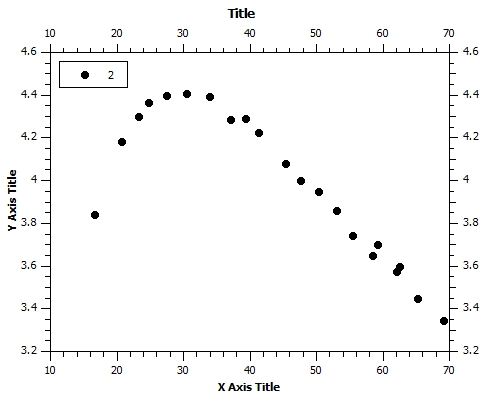
\includegraphics[width=0.6\linewidth, angle=0]{nudes/Leistung-Lastwiderstand-Diagramm.jpg}
    \caption{Leistung-Lastwiderstand-Diagramm}
    \label{fig:LeistungLastwiderstandDiagramm}
\end{figure}

\noindent
Die bereits im zweiten Aufgabenpunkt geforderten Parameter wurden auch hier mittels Formeln \ref{eq:Scheinleistung}, \ref{eq:Leistungsfaktor}, \ref{eq:Blindleistung}, \ref{eq:Verlustleistung}, \ref{eq:Wirkleistung} und \ref{eq:Wirkungsgrad} und den Werten aus Tabelle \ref{tab:messwerteOhmInduktiv} berechnet. Einige Werte wurden auch der Tabelle \ref{tab:berechnungenRPotP2} entnommen, wobei in beiden Fällen nur jene aus dem Maximum verwendet wurden.

\begin{table}[H]
    \centering
    \caption{Berechnungen Ohm'sche-Induktive Last}
    \label{tab:BerechnungenOhmInd}
    \begin{tabular}{| l | l | l | l | l | l |}
        \hline
        $P_{S1}$ / W & $P_{Q1}$ / W & $cos(\Phi)$ / & $P_{V}$ / W & $P_{2}$ / W & $\eta$ / \\
        \hline
        32 $\pm$ 3 & 29.8 $\pm$ 3.3 & 0.37 $\pm$ 0.04 & 7.39 $\pm$ 0.15 & 4.41 $\pm$ 0.14 & 0.374 $\pm$ 0.018 \\
        \hline
    \end{tabular}
\end{table}


\section{Diskussion} %diskussion der Unsicherheiten und Ergebnisse und evtl. verlgeich mit Literatur ------------------------------

Die berechneten Werte der Wirkleistung $P_{2}$ bilden wie erwartet eine Kurve, welche in etwa beim Punkt (30.6/4.41) ein Maximum besitzt. Da das Potentiometer in relativ großen Abständen verschoben wurde, könnte das tatsächliche Maximum auch im umliegenden Bereich dieses Punktes (aber auf jeden Fall zwischen den benachbarten Punkten) liegen.
Dieses Maximum kommt zustande, da der Sekundärstrom $I_{2}$ immer größer- und die Spannung $U_{R}$ immer kleiner wird. Dadurch, dass die beiden Größen multipliziert werden, ergibt sich ein Maximumspunkt. \newline

\noindent
Die exportierten Oszilloskopbilder weißen eine sehr ungewöhnliche Form des Primärstromes auf, dessen Verschulden nach gezieltem herumbasteln, messen und mit Hilfe von letztendlichem Ausschlussverfahren wahrscheinlich auf das Shunt fällt. Womöglich ist dieses-, oder das dazugehörige Oszilloskop-Interface (womöglich auf ein Kabel davon) defekt, was sich bei erneuter Versuchsdurchführung mit Ersatzgeräten vermeiden liese. Auch ein genauer Vergleich der Phasenverschiebung wird durch dieses Problem zusätzlich erschwert. \newline

\noindent
Da sich für eine solche Schaltung keinerlei Literaturwerte finden liesen, kann auch nur Schwer über die Richtigkeit der Berechnungen geurteilt werden. Jedoch wurden die Messwerte bereits während der Versuchsdurchführung mit den Erwartungswerten des Laborleiters verglichen, wodurch auf eine fehlerfreie Ausführung des Experimentes geschlossen werden kann.

\section{Zusammenfassung} %klare, übersichtliche vollständige beantwortung der Aufgabenstellung ------------------------------

Alle berechneten Werte und resultierende Diagramme werden in diesem Kaptiel noch einmal übersichtlich dargestellt und zusammengefasst. 

\subsection{Leerlauf}

\begin{table}[H]
    \centering
    \caption{Berechnungen Leerlauf}
    \label{tab:BerechnungenLeerlaufAW}
    \begin{tabular}{| l | l | l |}
        \hline
        $P_{S1}$ / W & $P_{Q1}$ / W & $cos(\Phi)$ / \\
        \hline
        27 $\pm$ 2 & 26 $\pm$ 3 & 0.26 $\pm$ 0.02 \\
        \hline
    \end{tabular}
\end{table}


\subsection{Ohm'sche Last sekundärseitig}

\begin{table}[H]
    \centering
    \caption{Berechnungen Leerlauf}
    \label{tab:BerechnungenLeerlaufAW}
    \begin{tabular}{| l | l | l | l | l | l |}
        \hline
        $P_{S1}$ / W & $P_{Q1}$ / W & $cos(\Phi)$ / & $P_{V}$ / W & $P_{2}$ / W & $\eta$ / \\
        \hline
        31.2 $\pm$ 2.1 & 25.5545 $\pm$ 3 & 0.58 $\pm$ 0.04 & 7.1 $\pm$ 0.6 & 10.9 $\pm$ 0.5 & 0.40 $\pm$ 0.04 \\
        \hline
    \end{tabular}
\end{table}


\subsection{Ohm'sche-induktive Last}

\begin{table}[H]
    \centering
    \caption{Berechnete Werte für $R_{Pot}$ und $P_{2}$}
    \label{tab:berechnungenRPotP2AW}
    \begin{tabular}{| l | l | l |}
        \hline
        Nr.  & $R_{Pot}$ / $\Omega$ & $P_{2}$ / W \\
        \hline
        1 & 69 $\pm$ 3 & 3.35 $\pm$ 0.14 \\
        2 & 69 $\pm$ 3 & 3.35 $\pm$ 0.14 \\
        3 & 65 $\pm$ 3 & 3.45 $\pm$ 0.14 \\
        4 & 62 $\pm$ 3 & 3.60 $\pm$ 0.14 \\
        5 & 62 $\pm$ 3 & 3.58 $\pm$ 0.14 \\
        6 & 59 $\pm$ 3 & 3.70 $\pm$ 0.14 \\
        7 & 58 $\pm$ 3 & 3.65 $\pm$ 0.14 \\
        8 & 55 $\pm$ 3 & 3.75 $\pm$ 0.14 \\
        9 & 52.9 $\pm$ 1.9 & 3.87 $\pm$ 0.14 \\
        10 & 50.4 $\pm$ 1.8 & 3.95 $\pm$ 0.14 \\
        11 & 47.6 $\pm$ 1.7 & 4.01 $\pm$ 0.14 \\
        12 & 45.4 $\pm$ 1.6 & 4.08 $\pm$ 0.14 \\
        13 & 41.3 $\pm$ 1.4 & 4.23 $\pm$ 0.14 \\
        14 & 39.4 $\pm$ 1.3 & 4.29 $\pm$ 0.14 \\
        15 & 37.1 $\pm$ 1.2 & 4.29 $\pm$ 0.14 \\
        16 & 33.9 $\pm$ 1.1 & 4.40 $\pm$ 0.14 \\
        \textbf{17} & \textbf{30.6 $\pm$ 1.0} & \textbf{4.41 $\pm$ 0.14} \\
        18 & 27.5 $\pm$ 0.9 & 4.40 $\pm$ 0.14 \\
        19 & 24.8 $\pm$ 0.8 & 4.37 $\pm$ 0.14 \\
        20 & 23.3 $\pm$ 0.8 & 4.30 $\pm$ 0.14 \\
        21 & 20.7 $\pm$ 0.7 & 4.19 $\pm$ 0.13 \\
        22 & 16.7 $\pm$ 0.6 & 3.84 $\pm$ 0.13 \\
        \hline
    \end{tabular}
\end{table}

\begin{figure}[H]
    \centering
    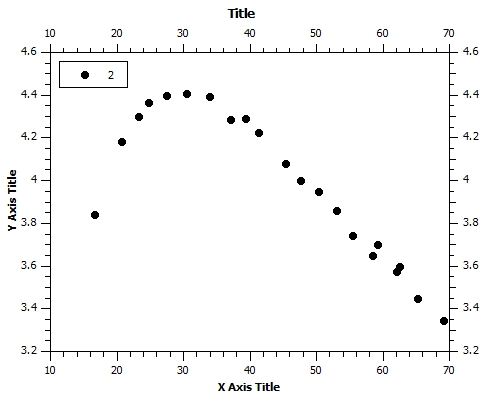
\includegraphics[width=0.6\linewidth, angle=0]{nudes/Leistung-Lastwiderstand-Diagramm.jpg}
    \caption{Leistung-Lastwiderstand-Diagramm}
    \label{fig:LeistungLastwiderstandDiagrammAW}
\end{figure}

\begin{table}[H]
    \centering
    \caption{Berechnungen Ohm'sche-Induktive Last}
    \label{tab:BerechnungenOhmIndAW}
    \begin{tabular}{| l | l | l | l | l | l |}
        \hline
        $P_{S1}$ / W & $P_{Q1}$ / W & $cos(\Phi)$ / & $P_{V}$ / W & $P_{2}$ / W & $\eta$ / \\
        \hline
        32 $\pm$ 3 & 29.8 $\pm$ 3.3 & 0.37 $\pm$ 0.04 & 7.39 $\pm$ 0.15 & 4.41 $\pm$ 0.14 & 0.374 $\pm$ 0.018 \\
        \hline
    \end{tabular}
\end{table}



\section{Anhang}



\printbibliography[heading=bibintoc]
\end{document}
